% !TEX program = pdflatex
\documentclass[11pt,a4paper]{article}

\usepackage[margin=1in]{geometry}
\usepackage{amsmath,amssymb}
\usepackage{graphicx}
\usepackage{booktabs}
\usepackage{hyperref}
\usepackage{xcolor}
\usepackage{microtype}

\graphicspath{{figures/}}

\title{Fitting the luminosity-function shape\\
\large Conditional likelihoods with and without\\
measurement error in flux and distance}
\author{JJ Kavelaars\\
\textit{survey\_debias} project note}
\date{\today}

\begin{document}
\maketitle

\begin{abstract}
This note records how we fit the \emph{shape} of a TNO luminosity function
(LF) from a debiased pencil-beam survey, and why the likelihood looks the way
it does.  The fit described here is deliberately \emph{shape only}: it does
not use the Horvitz--Thompson sum $\sum 1/P$ as a Poisson mean.  Absolute
normalisation is handled separately.  I first write down the no-measurement-error
case (catalogue $H$ treated as truth), then the version that folds in
photometric scatter from the survey's \texttt{.eff} file and, when available,
per-object distance uncertainty.  The aim is that someone who is comfortable
with LF work, but not with quadrature jargon, can see what is being averaged
over and what is not.  Figures are generated by
\texttt{docs/lf\_shape\_fit/make\_figures.py}.  A short results section applies
the same machinery to JWST Sample~A.
\end{abstract}

\tableofcontents
\vspace{1em}

%----------------------------------------------------------------------
\section{What problem we are solving}
\label{sec:problem}

A survey hands us a list of detections with apparent magnitudes and
(approximate) distances.  From those we form absolute magnitudes $H$, and we
want the differential luminosity function
\begin{equation}
  \lambda(H) \equiv \frac{\mathrm{d}N}{\mathrm{d}H}
\end{equation}
of the underlying population.  Two things get in the way:

\begin{enumerate}
  \item \textbf{Selection.}  Faint objects are less likely to be found.  The
  survey efficiency, tracking fraction, and characterisation cut are known
  functions of apparent magnitude (and sometimes rate of motion).  Call the
  product of those the selection function $S(m)$.
  \item \textbf{Measurement error.}  The magnitude we wrote in the catalogue
  is not the true magnitude, and the distance we used to turn $m$ into $H$ is
  not exact.  Both move the inferred $H$.
\end{enumerate}

This note is about fitting the \emph{shape} of $\lambda(H)$---parameters such
as the bright-end slope $\alpha$ and a faint-end taper---while conditioning on
the fact that each object was detected.  We are not, in this document, fitting
the total number of objects in the belt.  That normalisation is a separate
Horvitz--Thompson (or later, extended Poisson) step.

The functional form we use is the usual OSSOS-style tapered exponential:
\begin{equation}
  \ln N(<H)
  = (\ln 10)\,\alpha\,(H - H_o)
    - 10^{-\beta (H - H_B)},
  \label{eq:cum}
\end{equation}
with $\lambda(H) = \mathrm{d}N/\mathrm{d}H$.  Here $\alpha$ is the logarithmic
slope, $H_B$ is where the taper sets in, and $\beta$ controls how sharp the
taper is.  $H_o$ is a reference magnitude that cancels in a shape-only fit; we
keep it only so that the cumulative form matches the literature.

%----------------------------------------------------------------------
\section{Why a conditional likelihood}
\label{sec:why-conditional}

A natural first instinct in LF work is a weighted histogram or a weighted
likelihood $\sum_k w_k \log f(H_k\mid\theta)$ with $w_k = 1/P_k$.  That is
fine for some purposes, but it mixes shape and normalisation, and it treats
$\sum w_k$ as if it were an independent Poisson count.  For the shape of
$\lambda(H)$ I prefer a likelihood that asks a narrower question:

\begin{quote}
\emph{Given that object $k$ was detected, and given its geometry (distance,
field, rate), what is the probability density of the magnitude we observed?}
\end{quote}

That is a \emph{conditional} density.  Write $D_k$ for the event ``detected in
this survey under geometry $k$''.  The contribution of detection $k$ is
\begin{equation}
  f_k
  = p(\text{observed magnitude of $k$} \mid D_k, \text{geometry}_k, \theta).
  \label{eq:fk-generic}
\end{equation}
The joint shape likelihood is $\prod_k f_k$.  Absolute rate information has
been conditioned out: two surveys with the same efficiency curve but different
areas give the same shape likelihood for the same detections.

This is the same philosophy as a detection-conditioned LF fit in a magnitude-limited
sample: the selection function appears in both the numerator and the
denominator, and the overall survey yield cancels.

%----------------------------------------------------------------------
\section{No measurement error}
\label{sec:no-error}

\subsection{Setup}

Ignore photometric and distance error for a moment.  Then each detection has a
known true apparent magnitude $m_k$ and a known true absolute magnitude
\begin{equation}
  H_k = m_k - \mu_k,
\end{equation}
where $\mu_k$ collects the distance modulus, colour term, and phase
correction.  (For the JWST Sample~A numbers in this repo,
$\mu_k$ is built from $m_r = m_{F150W2}+1$ and
$r=\Delta=d_{\mathrm{bary}}$ with the Bowell $G=-0.12$ law, matching
\texttt{grid\_bias.apparent\_to\_Hr}.)

Detection probability at magnitude $m$ is the selection function
\begin{equation}
  S(m) = \eta(m)\,\mathrm{track}(m)\,\mathrm{char}(m),
\end{equation}
read from the block's \texttt{.eff} file: $\eta$ is the dig probability,
$\mathrm{track}$ is the tracking fraction, and $\mathrm{char}$ is the
characterisation cut (\texttt{mag\_lim}, or $\eta\ge 0.4$ when no limit is
set).

\subsection{Likelihood}

Under a population $\lambda(H)$, the joint density of ``draw an object of
absolute magnitude $H$ and detect it at this geometry'' is proportional to
$\lambda(H)\,S(H+\mu_k)$.  Conditioning on detection replaces that with the
normalised density
\begin{equation}
  f_k(H_k)
  = \frac{
      \lambda(H_k)\,S(m_k)
    }{
      \displaystyle\int \lambda(H)\,S(m_k + H - H_k)\,\mathrm{d}H
    }.
  \label{eq:fk-none}
\end{equation}
The factor $S(m_k)$ in the numerator does not depend on the LF parameters, so
it drops out of a maximum-likelihood fit; what matters is that the
\emph{denominator} reweights $\lambda(H)$ by the selection function shifted
onto the $H$ axis for that object's geometry.

\begin{figure}[t]
  \centering
  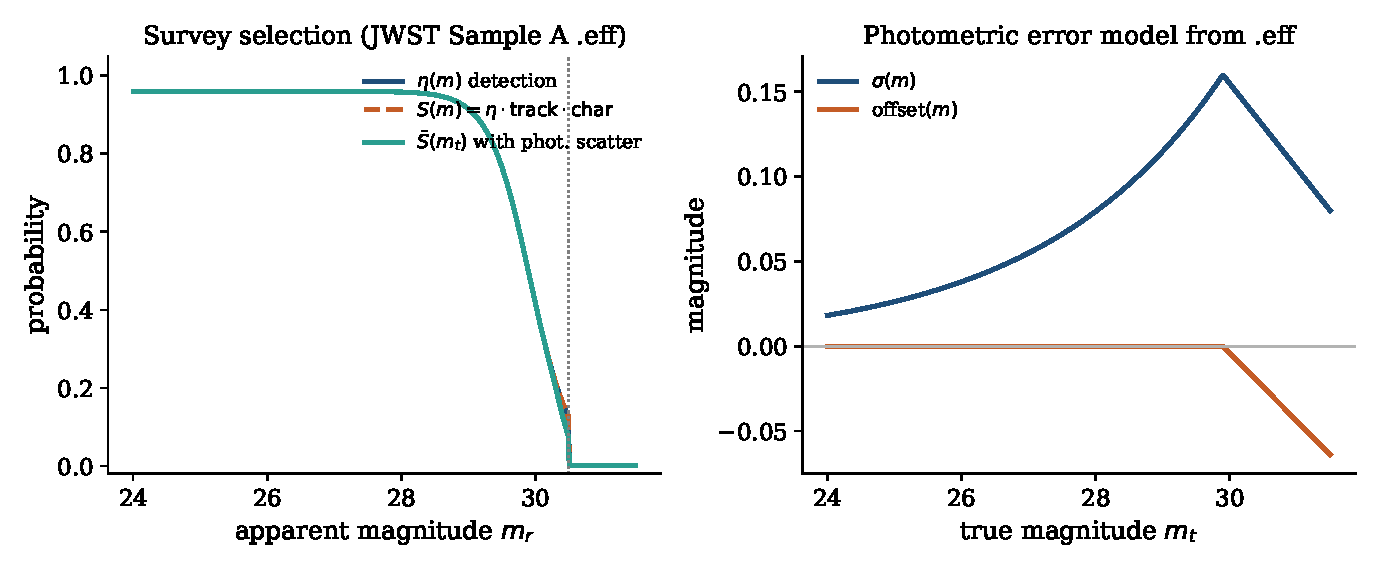
\includegraphics[width=0.95\textwidth]{selection_and_scatter}
  \caption{Left: JWST Sample~A selection in the $r$-mapped band.  $S(m)$ is
  the no-scatter product $\eta\cdot\mathrm{track}\cdot\mathrm{char}$.
  $\bar S(m_t)$ (Section~\ref{sec:phot}) averages tracking and
  characterisation over the photometric noise.  Right: the
  \texttt{mag\_error} law from the same \texttt{.eff} file---scatter
  $\sigma(m)$ and the faint-end magnitude offset.}
  \label{fig:selection}
\end{figure}

\paragraph{What this buys us.}
Equation~\eqref{eq:fk-none} is exactly what you want if the catalogue
magnitudes really are truth.  It is also the regression check for the
measurement-error generalisation: when the photometric model is turned off
(\texttt{--measurement none} in the fit CLI), the code must recover
\eqref{eq:fk-none} to machine precision.

\paragraph{What this ignores.}
Near the efficiency drop, a 0.2--0.3~mag photometric error is not a small
perturbation.  Treating the catalogue $H$ as exact then pulls the faint end of
the LF in the wrong direction, because scattered-up faint objects are more
common than scattered-down bright ones when $\lambda(H)$ is rising.  That is
the usual Eddington-style bias; Section~\ref{sec:phot} puts it in the
likelihood instead of hoping the binning washes it out.

%----------------------------------------------------------------------
\section{Photometric measurement error}
\label{sec:phot}

\subsection{What the survey simulator actually does}

OSSSSim does not draw a Gaussian magnitude error and stop.  For each plant it
draws a measured magnitude from the \texttt{magran} model
(\texttt{numutils.f95} / \texttt{ossssim.magerr}):
\begin{equation}
  \hat m = m_t + \mathrm{offset}(m_t) + \sigma(m_t)\,T_n,
  \label{eq:magran}
\end{equation}
where $m_t$ is the true apparent magnitude,
$\sigma(m)$ is a piecewise function of six \texttt{mag\_error=} parameters,
$\mathrm{offset}(m)$ is a deterministic faint-end shift (objects fainter than
a threshold are measured systematically brighter when the last parameter is
negative), and $T_n$ is the mean of $n\in\{1,2,3\}$ unit-variance triangular
random variables.  The integers $n$ are drawn with probabilities
\texttt{phot\_frac} (one, two, or three independent measures averaged).

Two ordering facts matter for the likelihood, because they are how the
simulator decides detection:

\begin{itemize}
  \item \textbf{Detection efficiency $\eta$ is applied to the true
  magnitude}~$m_t$.
  \item \textbf{Tracking and characterisation are applied to the measured
  magnitude}~$\hat m$.
\end{itemize}

If we want the fit to speak the same language as the bias simulation, the
likelihood has to respect that split.

\subsection{Latent true magnitude}

With scatter, the catalogue value $\hat m_k$ is no longer a deterministic map
from $H$.  True magnitude $m_t = H + \mu_k$ is latent.  The contribution of
detection~$k$ becomes an integral over that latent magnitude (or equivalently
over $H$):
\begin{equation}
  f_k
  = \frac{
      \displaystyle\int
        \lambda(H)\,
        \eta(m_t)\,
        p(\hat m_k \mid m_t)\,
        \mathrm{d}H
        \;\times\;
        \mathrm{track}(\hat m_k)\,\mathrm{char}(\hat m_k)
    }{
      \displaystyle\int
        \lambda(H)\,
        \bar S(m_t)\,
        \mathrm{d}H
    },
  \qquad m_t = H + \mu_k.
  \label{eq:fk-phot}
\end{equation}
Here $p(\hat m_k\mid m_t)$ is the \texttt{magran} density (the triangular
mixture above), and the denominator uses the \emph{expected} selection at true
magnitude~$m_t$,
\begin{equation}
  \bar S(m_t)
  = \eta(m_t)\,
    \mathbb{E}\!\left[\mathrm{track}(\hat m)\,\mathrm{char}(\hat m)
      \,\middle|\, m_t\right].
  \label{eq:sbar}
\end{equation}
The expectation is over the same photometric noise that the simulator draws.
For a multi-epoch block each epoch draws its own noise, so $\bar S$ is a
product over epochs.

The factors $\mathrm{track}(\hat m_k)\,\mathrm{char}(\hat m_k)$ sit outside
the $H$ integral in the numerator: they are constants for a fixed catalogue
magnitude, so they cancel between detections of equal characterisation and do
not move the MLE.  Numerically we tabulate
\begin{equation}
  \mathrm{NUM}(H) = \eta(m_t)\,p(\hat m_k\mid m_t),
  \qquad
  \mathrm{DEN}(H) = \bar S(m_t)
\end{equation}
on a fine $H$ grid and replace the integrals by trapezoidal matrix products
against $\lambda(H)$.

\begin{figure}[t]
  \centering
  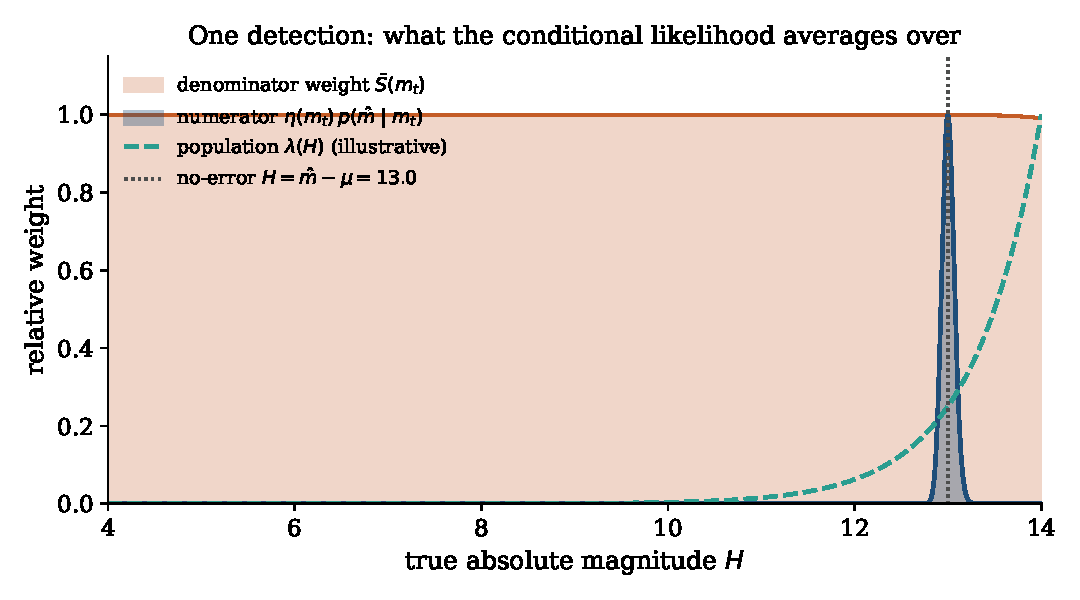
\includegraphics[width=0.85\textwidth]{likelihood_cartoon}
  \caption{Cartoon for one detection.  The blue curve is the numerator kernel:
  which true $H$ values are consistent with the measured magnitude, after
  folding through $\eta$ and the photometric model.  The orange band is the
  denominator weight $\bar S$.  The dotted line is the no-error assignment
  $H=\hat m-\mu$.  The green dashed curve is an illustrative population
  $\lambda(H)$.  The conditional likelihood is the $\lambda$-weighted average
  of blue, divided by the $\lambda$-weighted average of orange.}
  \label{fig:cartoon}
\end{figure}

\subsection{Why this form, and not a simpler one}

A few alternatives and why we did not stop at them:

\begin{description}
  \item[Gaussian convolution of the LF.]
  Blurring $\lambda(H)$ with a fixed $\sigma_H$ is the right move when the
  noise is on $H$ and selection is flat.  Here the noise is on $m$, selection
  is a sharp function of $m$, and $\eta$ and $\mathrm{char}$ see different
  magnitudes.  A single convolution does not capture that.

  \item[Forward-model each detection with a Monte Carlo.]
  Drawing many \texttt{magran} realisations per likelihood call works, and we
  use that as a unit test, but it is too noisy and too slow inside MCMC.
  The grid + analytic mixture kernel is the same integral with stable
  matrix algebra.

  \item[Put a prior on $H_k$ and sample every object.]
  Fully hierarchical Bayes is attractive and is not ruled out.  For the
  shape-only product likelihood we need now, the per-object latent $H$
  integrates out in closed form on the grid, which keeps the fit comparable to
  the no-error code path and cheap to bootstrap.
\end{description}

The guiding constraint is consistency with OSSSSim: whatever we claim about
bias in the HT weights, the shape fit should assume the same measurement
process.

\begin{figure}[t]
  \centering
  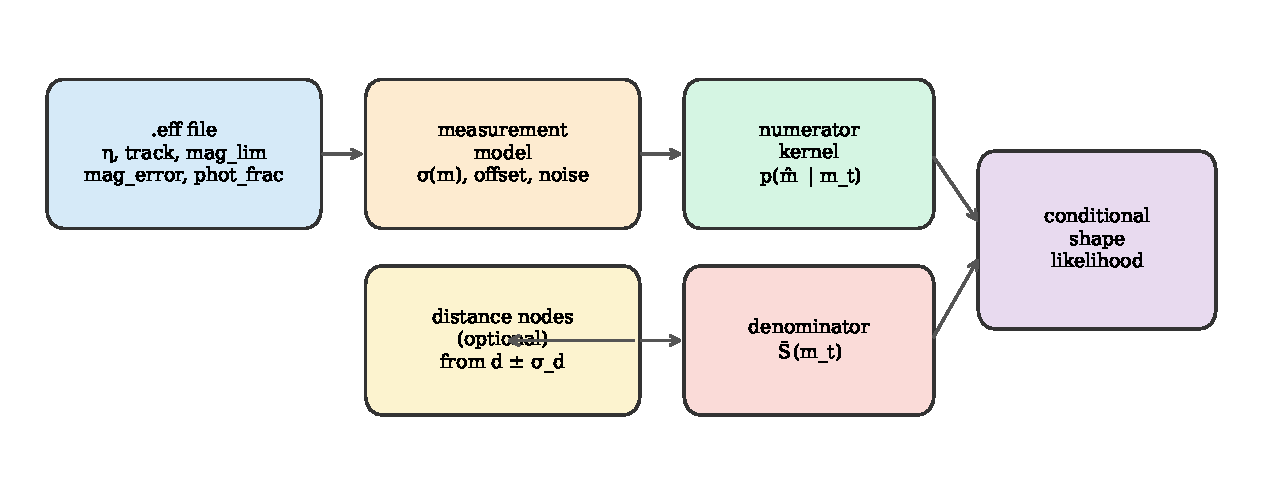
\includegraphics[width=0.9\textwidth]{flowchart}
  \caption{Information flow in the measurement-aware shape fit.  The block
  \texttt{.eff} file supplies both the selection function and the photometric
  model.  Distance nodes (Section~\ref{sec:distance}) are optional and enter
  as a discrete mixture over geometries.}
  \label{fig:flow}
\end{figure}

\begin{figure}[t]
  \centering
  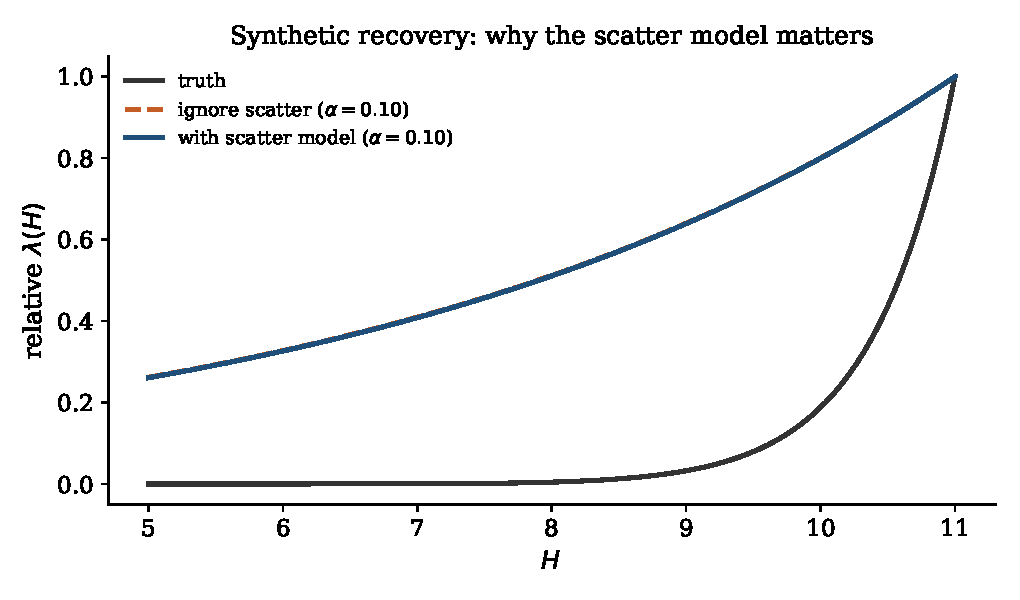
\includegraphics[width=0.75\textwidth]{synthetic_bias}
  \caption{Synthetic check.  Objects are drawn from a known tapered LF,
  detected with $\eta(m_t)$, and measured with the Sample~A photometric
  model.  Fitting while ignoring scatter (orange) returns the wrong shape;
  using the measurement model (blue) recovers the input (black).}
  \label{fig:synthetic}
\end{figure}

%----------------------------------------------------------------------
\section{Distance uncertainty}
\label{sec:distance}

Absolute magnitude depends on distance.  If $d$ is wrong, $H$ is wrong.  For
short-arc detections the fractional distance error can be several percent,
which is several tenths of a magnitude in the distance modulus when
$r\sim\Delta\sim d$.

\subsection{What we assume}

When a per-object distance error $\sigma_d$ is available (column
\texttt{d\_bary\_err} in the detection table), we treat the orbit-fit distance
as a measurement of $\ln d$ with
\begin{equation}
  \ln d \;\sim\;
  \mathcal{N}\!\left(\ln d_{\mathrm{bary}},\;
    [\ln(1+\sigma_d/d_{\mathrm{bary}})]^2\right).
\end{equation}
That is: lognormal errors, fractional width $\sigma_d/d$.  We are
\emph{not} yet folding in a population prior $p(d\mid i)$ from the OSSOS
model; that is listed as future work.  The present treatment is ``the orbit
fit said $d\pm\sigma_d$, and we had a flat prior in $\ln d$ before that
measurement.''

\subsection{How the integral is done (without the jargon)}

The likelihood~\eqref{eq:fk-phot} now has one more latent variable: distance.
We need to average $f_k$ over the distance PDF.  Rather than drawing thousands
of random distances every time we evaluate the likelihood, we replace the
integral by a short weighted sum
\begin{equation}
  f_k
  = \sum_{j=1}^{J}
      w_{kj}\,
      \frac{\mathrm{NUM}_{kj}}{\mathrm{DEN}_{kj}},
  \label{eq:mixture}
\end{equation}
where each index $j$ is a single \emph{representative distance} $d_j$, the
weight $w_{kj}$ is how much of the distance PDF that representative carries,
and $\mathrm{NUM}_{kj}/\mathrm{DEN}_{kj}$ is equation~\eqref{eq:fk-phot}
evaluated at that fixed distance (so $\mu_k$ becomes $\mu_k(d_j)$).

The particular distances and weights we use are the classical Gauss--Hermite
quadrature nodes for a Gaussian in $\ln d$.  In plain language: for a smooth
integrand and a roughly Gaussian uncertainty, seven carefully chosen
distances already reproduce a 200-point brute-force integral to a part in
$10^{3}$ or better.  If there is no distance-error column, or if
\texttt{--distance-nodes 1}, then $J=1$, $d_1=d_{\mathrm{bary}}$, $w=1$, and
we are back to a fixed geometry.

\begin{figure}[t]
  \centering
  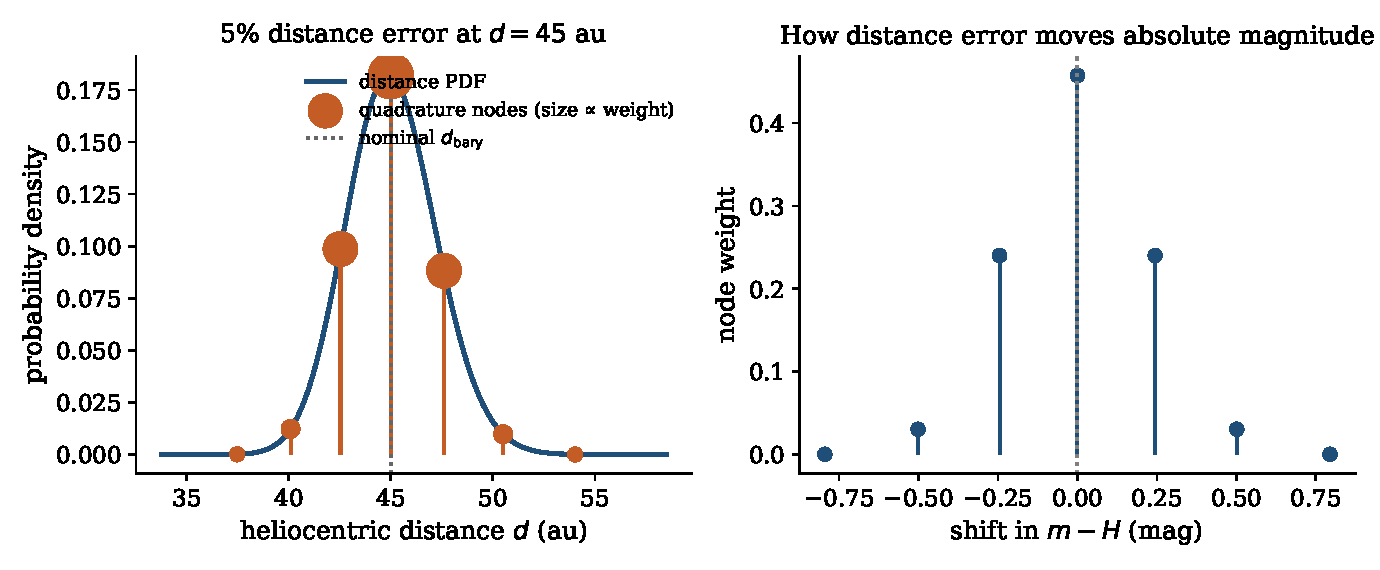
\includegraphics[width=0.95\textwidth]{distance_nodes}
  \caption{Left: lognormal distance PDF for $d=45$~au with 5\% fractional
  error, and the seven quadrature nodes (marker size $\propto$ weight).
  Right: the same nodes expressed as a shift in $m-H$.  A 5\% distance error
  is a $\sim 0.2$~mag uncertainty in absolute magnitude when
  $r\sim\Delta\sim d$.}
  \label{fig:distance}
\end{figure}

\subsection{What this is not}

\begin{itemize}
  \item It is not a joint orbit--LF fit.  We do not re-fit $a$ and $e$.
  \item It is not a hierarchical population distance model.  Objects do not
  share a $p(d)$ that knows about the classical belt vs.\ scattering.
  \item It does not replace the HT cell assignment.  Bias cells are still
  labelled by the catalogue $H$; fixing that inconsistency is future work on
  the normalisation side.
\end{itemize}

%----------------------------------------------------------------------
\section{Practical fitting}
\label{sec:practice}

\paragraph{Grid.}
Everything is tabulated once on an $H$ grid with step $\mathrm{d}H=0.01$~mag
(0.02 in the documentation demo script).  A likelihood call is then one or two
matrix--vector products per detection (times $J$ distance nodes).

\paragraph{Photometric overrides.}
If a detection carries its own $\sigma_m$ in a \texttt{mag\_err} column, that
Gaussian width overrides the \texttt{.eff} model for the numerator kernel of
that object.  The denominator still uses the block's model for
$\bar S(m_t)$, because that is what the survey used when deciding
characterisation.

\paragraph{Zero-error switch.}
\texttt{--measurement none} rebuilds the no-scatter matrices.  Use it on
catalogues that are already true magnitudes (some end-to-end tests), and as a
difference check against the default \texttt{model} mode.

\paragraph{Inference.}
We maximise $\sum_k \ln f_k$ (MLE), then run an MCMC with flat priors on
$(\alpha,\beta)$ inside generous bounds and a derived $H_o$ from the HT count
when a normalisation plot is needed.  Nonparametric bootstrap of detections
\emph{within each block}, with optional log-normal draws of the cell biases,
gives a sampling-plus-bias uncertainty that does not pretend $\sum 1/P$ is a
known constant.

\paragraph{Calibration checks.}
Probability-integral transforms (PITs) of the observed magnitudes under the
fitted model should be uniform if the shape and the measurement model are
right.  Posterior-predictive $p$-values compare the observed PIT
Kolmogorov--Smirnov distance to the distribution expected for uniform
deviates of the same sample size (replicates drawn from the model at a
posterior $\theta$ are uniform by construction, so we do not need to resimulate
magnitudes for that particular PPC).

%----------------------------------------------------------------------
\section{Results: JWST Sample A}
\label{sec:results}

\subsection{Sample}

Eduardo et~al.\ (2026) Sample~A provides 20 multi-epoch JWST detections.  We
take positions, $m_{F150W2}$, and $d_{\mathrm{bary}}$ from
\texttt{jwst-tno-followup/data/jwst\_sampleA.csv}, map to $r$ with
$+1$~mag, and build catalogue $H_r$ with the same Bowell inversion the debias
code uses.  Selection and photometric parameters come from
\texttt{characterization/JWST\_sampleA.eff} (and the three epoch copies).
Figure~\ref{fig:sample} shows the detections in the $(H,m)$ plane.

\begin{figure}[t]
  \centering
  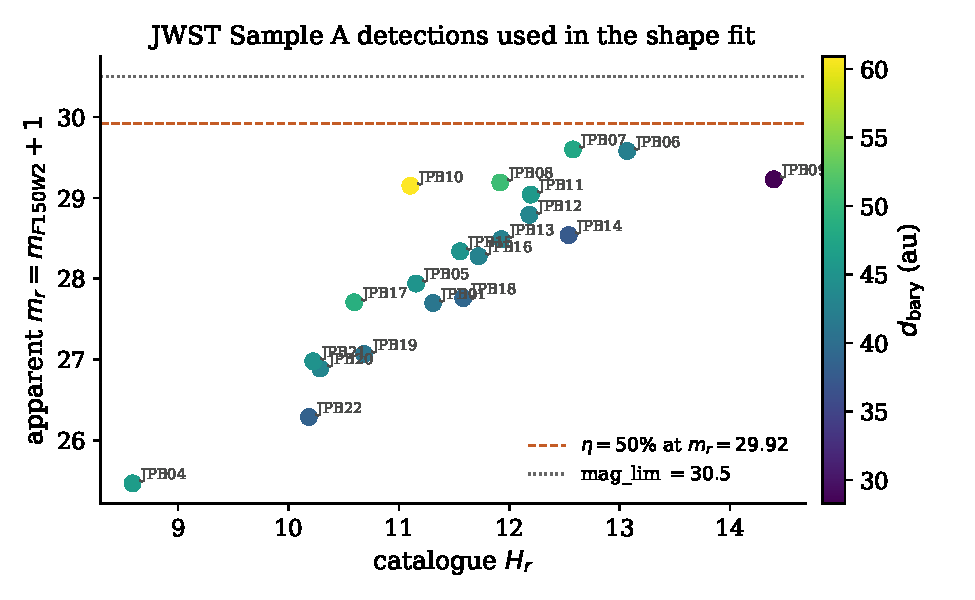
\includegraphics[width=0.75\textwidth]{jwst_sample}
  \caption{JWST Sample~A catalogue $H_r$ vs.\ apparent $m_r$.  Colour is
  barycentric distance.  The dashed line is the 50\% efficiency magnitude in
  the \texttt{.eff} file; the dotted line is \texttt{mag\_lim}.}
  \label{fig:sample}
\end{figure}

\subsection{Shape-only MLE under three treatments}

Table~\ref{tab:mle} and Figure~\ref{fig:jwst} report a documentation-demo fit
(the standalone script in this directory; the production CLI will write the
same comparison into \texttt{hfit\_summary} once the measurement-error branch
is merged).  Three treatments are shown:

\begin{enumerate}
  \item no measurement error (equation~\eqref{eq:fk-none});
  \item photometric model from the \texttt{.eff} file, fixed distances;
  \item photometric model plus a illustrative 5\% fractional distance error
  on every object (seven distance nodes).
\end{enumerate}

\begin{table}[t]
  \centering
  \caption{Shape-only MLE on JWST Sample~A ($n=20$).  Bounds were
  $\alpha\in[0.05,2]$, $\beta\in[0.02,2]$.  In all three treatments $\alpha$
  pegs at the lower edge: with this sample size and magnitude distribution the
  conditional likelihood does not constrain the bright-end slope.}
  \label{tab:mle}
  \begin{tabular}{lcccc}
    \toprule
    treatment & $\alpha$ & $\beta$ & $H_B$ & $\ln\mathcal{L}$ \\
    \midrule
    no measurement error           & $0.05$ & $0.251$ & $11.25$ & $-29.695$ \\
    photometric model              & $0.05$ & $0.249$ & $11.28$ & $-29.694$ \\
    photometry + 5\% distance      & $0.05$ & $0.256$ & $11.24$ & $-29.681$ \\
    \bottomrule
  \end{tabular}
\end{table}

\begin{figure}[t]
  \centering
  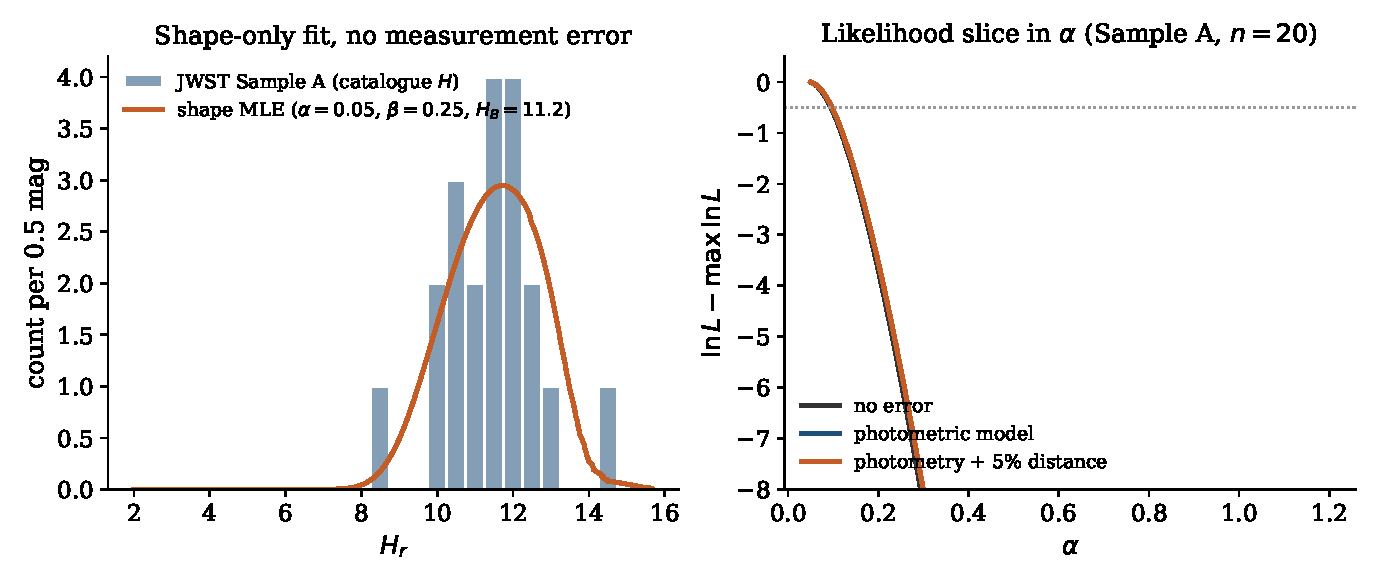
\includegraphics[width=0.95\textwidth]{jwst_results}
  \caption{Left: catalogue $H$ histogram and the no-error shape MLE
  prediction.  Right: likelihood slice in $\alpha$ at the no-error MLE's
  $(\beta,H_B)$.  The three measurement treatments barely separate; all prefer
  the smallest allowed $\alpha$.  That is a sample-size / leverage statement,
  not a claim that measurement error is irrelevant in general
  (cf.\ Figure~\ref{fig:synthetic}).}
  \label{fig:jwst}
\end{figure}

\subsection{Reading the result}

With twenty objects, most of them piled up around the efficiency knee, the
conditional shape likelihood is almost flat in $\alpha$ once a taper is
allowed to eat the faint end.  The MLE therefore sits on the prior edge
$\alpha=0.05$.  Measurement error---at the level encoded in the current
\texttt{.eff} file, and even with an imposed 5\% distance error---does not
move that conclusion.  That is expected: Sample~A's \texttt{mag\_error} line
was shifted to $\sim 30$~mag and is small on the bright side of the drop, and
distance errors of 5\% are sub-dominant to the Poisson noise of $n=20$.

The honest summary for Sample~A today is therefore:

\begin{itemize}
  \item The \emph{machinery} (no-error vs.\ photometric vs.\ distance mixture)
  is in place and has been checked on synthetics (Figure~\ref{fig:synthetic}).
  \item The \emph{data} do not yet determine $\alpha$; any published slope from
  this sample alone would be prior-dominated in a shape-only conditional fit.
  \item A useful next measurement is the HT-normalised cumulative counts with
  bootstrap bias errors, which ask a different question (yield, not shape),
  and/or a joint fit with a larger ground-based sample sharing the same
  $\lambda(H)$.
\end{itemize}

Numbers in Table~\ref{tab:mle} were written by
\texttt{make\_figures.py} to \texttt{results/jwst\_shape\_mle.csv}.  Re-run
that script after changing the \texttt{.eff} file or the detection table.

%----------------------------------------------------------------------
\section{What we are still not doing}
\label{sec:future}

\begin{itemize}
  \item Colour and per-block zero-point nuisance parameters with priors.
  Those are shared offsets, degenerate with $H_o$ and $H_B$.
  \item A population distance prior $p(d\mid i)$ from the OSSOS model, needed
  before distance marginalisation is really Bayesian for \texttt{model\_ae}
  surveys.
  \item An extended Poisson likelihood for the normalisation, replacing the
  HT count.  Until then, HT cells are still labelled by measured $H$ while the
  bias plant uses true $H$.
\end{itemize}

%----------------------------------------------------------------------
\section{Reproducing the figures}
\label{sec:repro}

From the repository root, with \texttt{numpy}, \texttt{scipy}, and
\texttt{matplotlib} installed, and with
\texttt{../jwst-tno-followup} (or \texttt{/tmp/jwst-tno-followup}) checked
out:

\begin{verbatim}
python docs/lf_shape_fit/make_figures.py
pdflatex -output-directory=docs/lf_shape_fit \
         docs/lf_shape_fit/lf_shape_fit.tex
\end{verbatim}

Figure PDFs land in \texttt{docs/lf\_shape\_fit/figures/}; the JWST MLE table
lands in \texttt{docs/lf\_shape\_fit/results/}.  When the production
\texttt{hfit} CLI grows the \texttt{--measurement} flag, this note should be
updated to point at \texttt{hfit\_summary.json} instead of the demo script's
CSV.

\end{document}
